% !TeX program = lualatex
\documentclass[a4paper,12pt,twoside]{article}
\usepackage{report}

\begin{document}
\thispagestyle{empty}
%\tikz[remember picture,overlay][t!] \node[opacity=3,inner sep=2pt] at (current page.center){\includegraphics[width=\paperwidth,height=\paperheight,keepaspectratio]{images/RHcoverphoto.jpg}};
%\clearpage


\begin{figure}[t!]
\centering
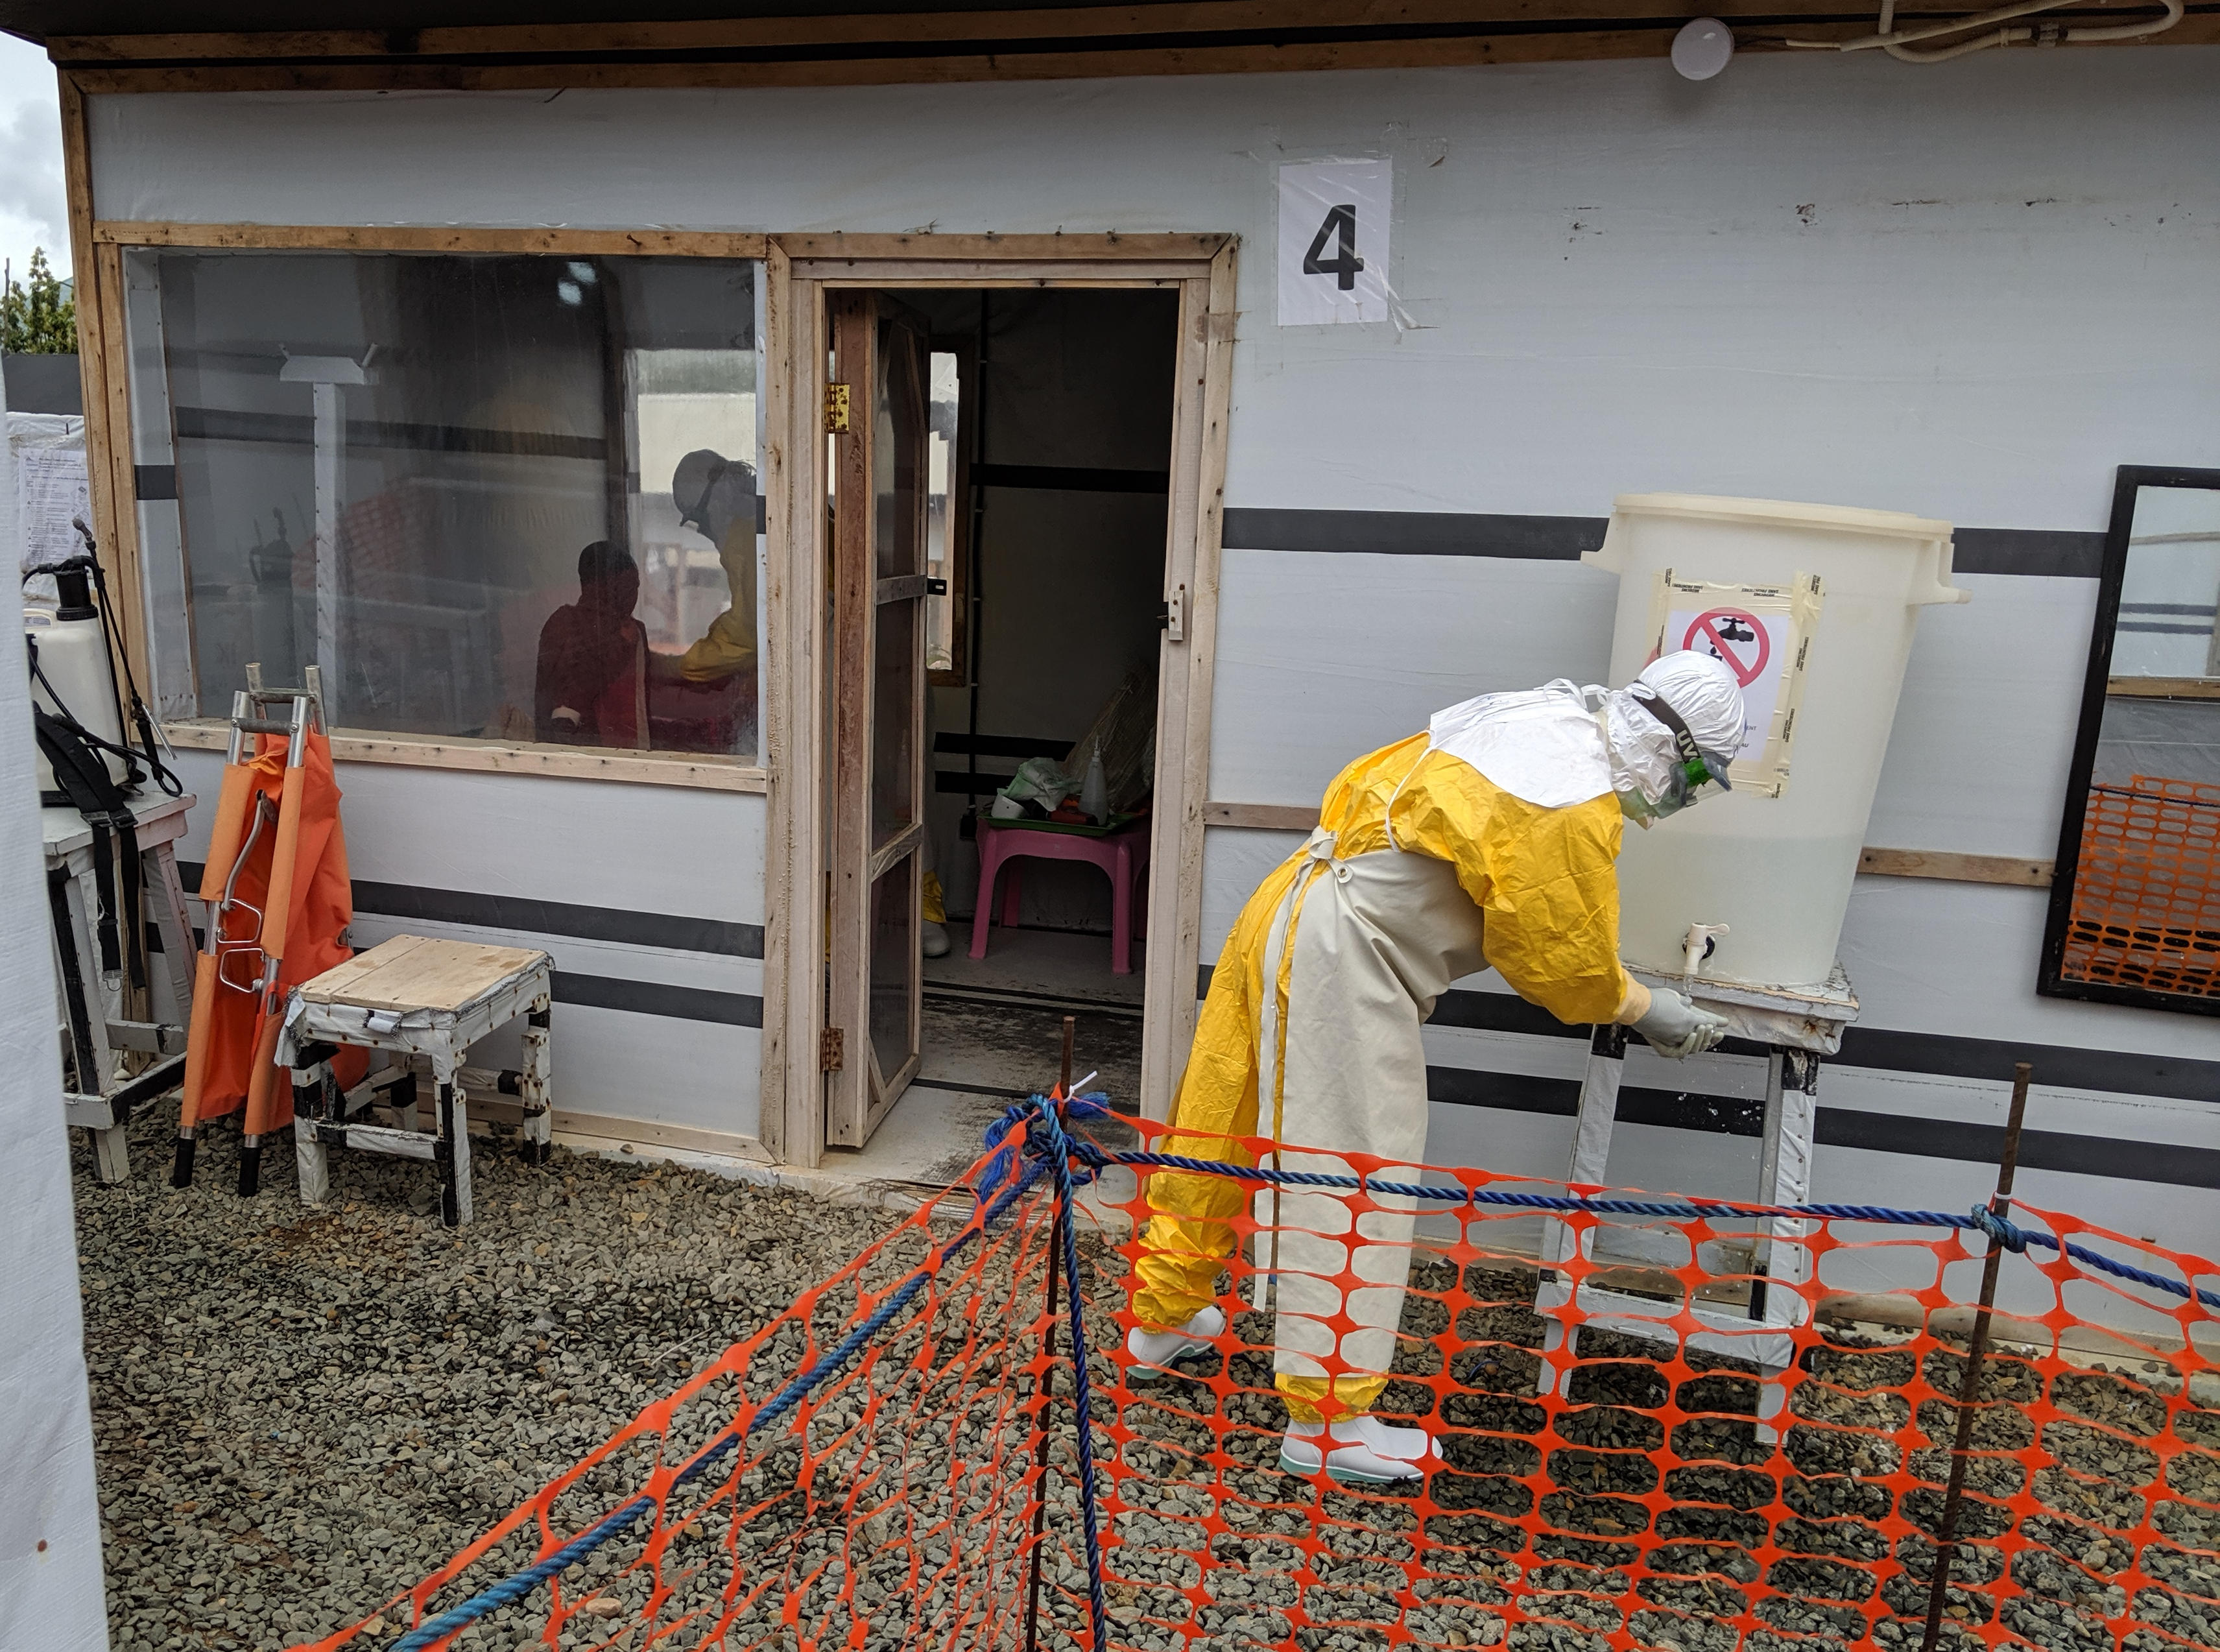
\includegraphics[width=\textwidth, height=12cm]{Medics_treating_patient_washing_hands_compressed.jpg}
\end{figure}

\begin{center}
  \huge \color{RHblue} \textbf {BUENDIA EBOLA MEDICAL RECORDS}

\textbf{Bunia, Ituri Province, Democratic Republic of the Congo, 2019}
\end{center}
\medskip


\begin{center}
  Ivan Gayton, Ka-Ping Yee, and Eric Perakslis
  \
  
\end{center}
\medskip
\begin{center}
\color{RHblue}\rule{\textwidth}{0.5cm}
\end{center}

\newpage
\newpage

% Reduce the spacing between Table of Contents items to get it down to 1 page

%\renewcommand{\baselinestretch}{1.0}\normalsize
\tableofcontents
%\renewcommand{\baselinestretch}{1.0}\normalsize

\newpage
\section{Summary of Current Status}
During a three-week visit to the Ebola-affected area of the Democratic Republic of the Congo in September and October 2019, the team was unable to deploy the system in Bunia---our intended site---due to an inability to obtain formal permission from the Congolese officials managing the Riposte (the locally-led coordination system for the Ebola response). 

However, the team was able to gather detailed user requirements from the medics on the ground, conduct training with local staff, provide demonstrations for local Riposte representatives, and implement fixes for technical issues that only revealed themselves once in the field. The team was also able to implement several new features and changes requested by the team in the field.

With support from the Emergency Coordinator of MSF-Switzerland in Goma, DRC, the inter-sectional legal department of MSF in Geneva, and the Riposte officials in Bunia, we have now obtained verbal agreement to deploy the system, and are in the process of seeking signature of a formal agreement to proceed. 

The team hopes to return to Bunia by mid-November to deploy the system. If the agreement is signed in time, we will do so.

\section{Next Steps}
\subsection{Technical Tasks}
The team is currently working on several improvements based on the experience and feedback in October in Bunia. Both Ka-Ping Yee (lead developer) and Schuyler Erle (primarily back-end dev) are working part-time on the system in anticipation of the upcoming deployment. 
\begin{itemize}
    \item Fixing an issue with the server clock that causes unexpected sync behavior
    \item Modifying the Treatment interface to choose route of administration before selecting the medication
    \item An updated profile
    \item A "none of the above" choice for multiple selects (and a bit of a general design re-think of negative reporting)
    \item A specific interface for managing perfusions
    \item Adding MSF stock codes to the treatment interface
    \item Improving the overall security, install procedure, backup and restore, and dashboard of the server
\end{itemize}

\subsection{Deployment Planning}
The Emergency Coordinator for MSF-Switzerland in Goma, Marc, is in discussions with Professor Steve Ahuka, the head of the Riposte in Goma, who would likely be the signatory for the permission. Julie Habran from the MSF Intersectional Legal department has prepared a proposed agreement, which Marc has shared with the Riposte and is following up with Professor Akuha. As soon as the permission is obtained:

\begin{itemize}
    \item Ping will travel to Bunia to resume the training and deployment. We hope this could happen as soon as the week of November 11th.
    \item Ivan will remain in Burkina Faso in a remote support role for the first week or two of the deployment to reduce both financial burn rate and burden on the field team. Once the initial deployment is done and stabilized, Ivan will likely travel to Bunia, take a handover from Ping, and remain for several weeks.
    \item If additional field support is needed, Eric will initiate visa process to travel to the field to support Ivan and the team.
\end{itemize}

\section{Progress on Permission}

The Ebola "Riposte" (response) is led by the Congolese government. This is different from the more common "Cluster" system where a United Nations agency coordinates efforts. Congolese officials make final decisions on all Ebola activities on a fairly granular level.

After seeing the system, local Riposte officials in Bunia (in particular Dr. Shoko, the local head of the Riposte in Bunia) were supportive and have been advocating to the 


\section{Opportunities}
\begin{itemize}
    \item Geneva Health Forum in March 2020
    \item MSF Scientific Days in London in May 2020
    \item Potential partnership with Epicentre on Ebola DRC and beyond
    \item Partnership with London School of Hygiene and Tropical Medicine
    \item Partnership with OpenDataKit consortium on health
    \item Possibility of publishing academic research on both the process and results of the project
    
\end{itemize}
\end{document}